
%% This file represents a sample first chapter of the main body of the dissertation
%%

% A first, optional argument in [ ] is the title as displayed in the table of contents
% The second argument is the title as displayed here.  Use \\ as appropriate in
%   this title to get desired line breaks
\chapter[Introduction]{Introduction}

\section{Background}
\section{Previous Work} % Literature Review?

Prior work in this field did xyz, and we need to write a line long enough so that we can see both the left and right hand margins.

Lorem ipsum, dolor sit amet consectetur adipisicing elit. Iure quod voluptatum cumque architecto tempora nobis dolorum vitae. Eius ipsa libero, \cite{matt_eg_1} rerum nesciunt voluptatum rem quis quos animi et sunt nihil.
Lorem ipsum, dolor sit amet consectetur adipisicing elit. Iure quod voluptatum cumque architecto tempora nobis dolorum vitae. Eius ipsa libero, rerum nesciunt voluptatum rem quis quos animi et sunt nihil.
Lorem ipsum, dolor sit amet consectetur adipisicing elit. Iure quod voluptatum cumque architecto tempora nobis dolorum vitae. Eius ipsa libero, rerum nesciunt voluptatum rem quis quos animi et sunt nihil.


Lorem ipsum, dolor sit amet consectetur adipisicing elit. Iure quod voluptatum cumque architecto tempora nobis dolorum vitae. Eius ipsa libero, rerum nesciunt voluptatum rem quis quos animi et sunt nihil.
\begin{enumerate}
  \item item 1
  
  \item item 2
  
  \item item 3
  
  \item item 4 
\end{enumerate}


\begin{figure}
  \centering
  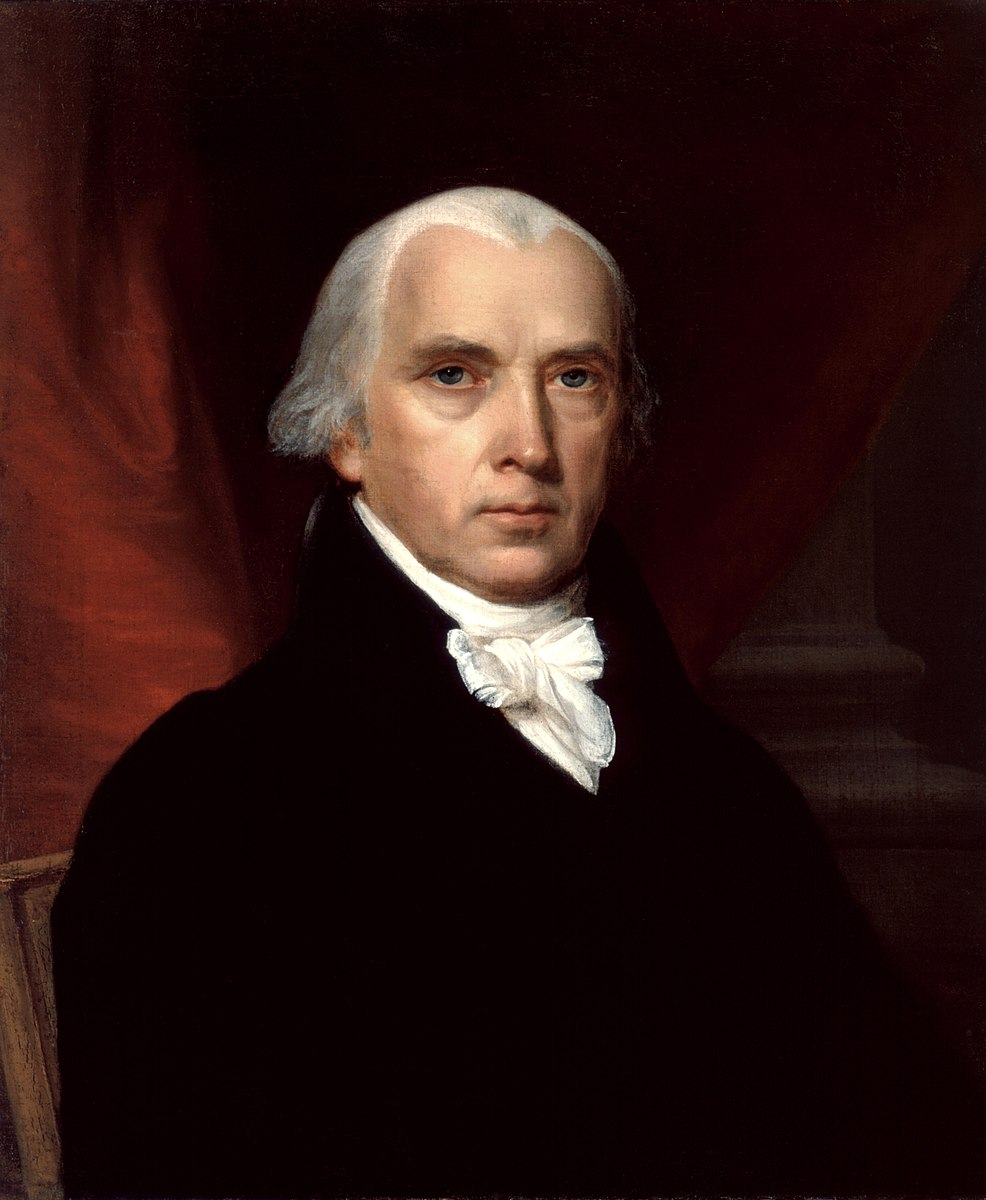
\includegraphics[scale=0.2]{figJamesMadison}
  \caption[An appropriate historical figure]{An appropriate historical figure.}

  % If you need more separation space between this figure and either another figure, or between
  %     the figure and the text, you can add figSpace as shown here.
  \figSpace
\end{figure}

\newpage

\subsection{A Subsection}

Important previous work was also provided by \cite{Shannon49}.  Here is a numbered equation:
\begin{equation}
    f_X(x) = \lambda e^{-\lambda x} u(x).
\end{equation}

Lorem ipsum, dolor sit amet consectetur adipisicing elit. Iure quod voluptatum cumque architecto tempora nobis dolorum vitae. Eius ipsa libero, rerum nesciunt voluptatum rem quis quos animi et sunt nihil.

\subsubsection{A subsubsection}

Lorem ipsum, dolor sit amet consectetur adipisicing elit. Iure quod voluptatum cumque architecto tempora nobis dolorum vitae. Eius ipsa libero, rerum nesciunt voluptatum rem quis quos animi et sunt nihil.

\paragraph{A paragraph}

Lorem ipsum, dolor sit amet consectetur adipisicing elit. Iure quod voluptatum cumque architecto tempora nobis dolorum vitae. Eius ipsa libero, rerum nesciunt voluptatum rem quis quos animi et sunt nihil.

\subparagraph{A subparagraph}

Lorem ipsum, dolor sit amet consectetur adipisicing elit. Iure quod voluptatum cumque architecto tempora nobis dolorum vitae. Eius ipsa libero, rerum nesciunt voluptatum rem quis quos animi et sunt nihil.



\begin{table}
  \centering
  \caption{A table}
  % Tabular environment goes AFTER the caption!
  \begin{tabular}{|c|c|c|}
    % after \\: \hline or \cline{col1-col2} \cline{col3-col4} ...
    \hline
    A & B & C \\\hline
    D & E & F \\\hline
    G & H & I \\
    \hline
  \end{tabular}

  % This adds separation space between this table and either another table, or between
  %     the table and the text.
  \tableSpace
\end{table}


\begin{table}
  \centering
  \caption{Another table}
  % Tabular environment goes AFTER the caption!
  \begin{tabular}{|c|c|c|}
    % after \\: \hline or \cline{col1-col2} \cline{col3-col4} ...
    \hline
    1 & 2 & 3 \\\hline
    4 & 5 & 6 \\\hline
    7 & 8 & 9 \\
    \hline
  \end{tabular}

  % This adds separation space between this table and either another table, or between
  %     the table and the text.
  \tableSpace
\end{table}
